\documentclass[10pt,twoside]{IEEEtran}
\providecommand{\keywords}[1]{\textbf{\textit{Keywords---}}#1}

\usepackage{alphalph}
\usepackage{graphicx}
\renewcommand\thesubsectiondis{\AlphAlph{\value{subsection}}.}% for the headings in the text

%opening
\title{Using a Genetic Algorithm to Optimize Heuristic Variables for Constraint Satisfaction Problems}
\author{Ryan Darras, Sudhanshu Semwal}

\begin{document}

\maketitle

\begin{abstract}
Constraint satisfaction problems (CSPs) consists of a set of objects \emph{V}, each with their own variables, and a set of constraints \emph{E} on the variables of the objects. To solve a CSP a state of \emph{V} must be found that satisfies every e ${\in }$ \emph{E}. CSPs often require a combination of heuristics and search algorithms to solve due to their high complexity and NP-hardness. Branch-and-Bound (BnB) algorithms are commonly used for solving NP-hard problems due to its nature of being a state space search. A BnB algorithm uses heuristics to optimize the upper and lower bounds, reducing the total amount of space searched to optimize efficiency. However, heuristics can often times decrease accuracy in favor of efficiency. Optimizing heuristic variables is also a challenge due to the complexity of the problems which prevents us from being able to statistically determine the optimal values.

We propose a genetic algorithm, implemented in the form of a NuGet package for the .NET framework, that will determine the optimal heuristic values for constraint satisfaction problems. 

\vspace{5mm}
\noindent \keywords{Constraint Satisfaction Problem, Branch-and-Bound, Heuristic, Genetic}
\end{abstract}

\section{Introduction}
CSPs, even if you don't know it, are problems that you interact with almost every day. Many researchers are studying CSPs and focusing on optimizing them because of how relevant they are in todays society. 

Everybody loves Amazon, the modern age option to shop in the comfort of home and have items shipped directly to the door step. However, most everybody does not understand the complexity behind managing such a massive operation. The Traveling Salesman Problem is a common lesson for undergraduate students to teach them the topic of NP-hard problems, but it is a small problem compared to what Amazon and other distributors have to deal with. In the United States alone, Amazon delivers millions of packages per day throughout thousands of cities. Each delivery driver works a scheduled shift anywhere from roughly four to ten hours a day, with many cities managing multiple drivers. Every single route needs to be planned as optimally as it can to have the availability of two-day shipping. They also need to consider shipping between warehouses that are on the opposite side of the country from one another. Without researchers designing effective algorithms to increase the efficiency of this massive problem, we wouldn't have the luxury of having our online purchases appearing on our doorstep in just a few days of the order. This is simply because of the massive complexity of their problem, which is why researching CSPs is so important.

Due to the potential NP-Hardness of many CSPs and their relationships that allow research to share across problems, they have been subject of profound study in both artificial intelligence and operations research. A solution to these problems can be found by using Branch-and-Bound (BnB) algorithms. BnB algorithms are a very common tool when solving NP-hard problems due to their nature to become an exhaustive search which will provide every possible answer. However, exhaustive BnB algorithms are incredibly inefficient but they can be heavily optimized by implementing a heuristic which determines if a branch cannot be a potential solution, in which case the branch is pruned. 

Due to the possible increase in efficiency, creating an efficient heuristic that accurately measures each branch is an incredibly important part of optimizing these problems. In this research, we propose a genetic algorithm that will determine the optimal heuristic values for any given CSP.

\section{Experimental Problems Background}
This research will focus on three example CSPs to perform tests and gather metrics. These are three very common CSPs, but they differ greatly when it comes to the heuristic variables which is why we are testing our genetic algorithm against them.

%\subsection{Traveling Salesman Problem}
%The generic NP-hard problem that has been used in examples all over the world to teach beginner computer scientists about complexity and optimality in mathematical problems. The problem consists of graph \emph{G} with vertices \emph{V} and edges \emph{E}. Given our traveling salesmen starts at vertex \emph{s ${\in}$ V}, he must travel to every other vertex \emph{${\forall}$x ${\in}$ \{V ${\mid}$ x ${\neq}$} v\} and return to starting vertex \emph{s}. Finding a solution to this problem is not difficult assuming you are not considering optimality, but finding an optimal solution has been proven NP-hard.

%\begin{figure}[h]
%	\centering
%	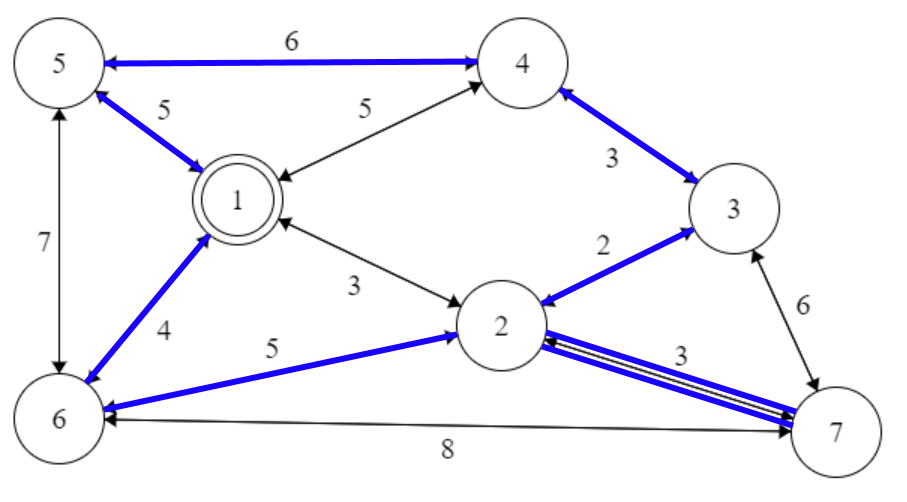
\includegraphics[width=0.9\linewidth]{../diagrams/tsp.png}
%	\caption{Example of solved Traveling Salesman Problem where vertex 1 is the starting and ending node, and the bold path is the optimal path.}
%	\label{TSP fig}
%\end{figure}

\subsection{Graph Coloring Problem}
Given constraints \emph{C} on a graph \emph{G = \{V, E\}}, the graph coloring problem (GCP) is to create an assignment of colors to vertices of the graph that meets the constraints in \emph{C}. Constraints are often similar to, ''Orange vertices may only connect via an edge to other orange vertices or blue vertices."

\begin{figure}[h]
	\centering
	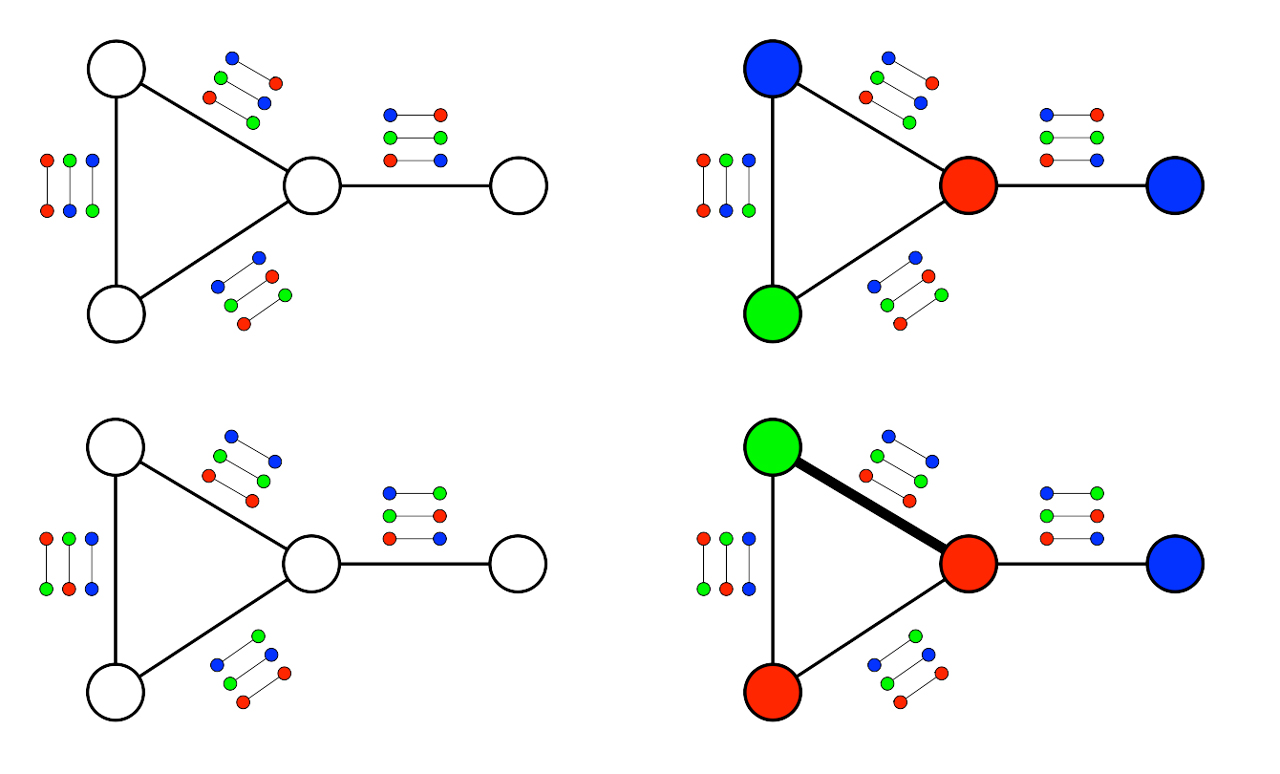
\includegraphics[width=0.7\linewidth]{../diagrams/GCP.jpg}
	\caption{Graphs that show the potential options of each edge to satisfy the constraints. The bottom right image demonstrates that certain constraints deem the problem impossible.}
	\label{GCP Fig}
\end{figure}

\subsection{n Queens Problem}
This problem consists of finding a state of an \emph{n} x \emph{n} chessboard with \emph{n} queens such that no two queens threaten each other. The complexity here arises when you consider that in chess a queen can move horizontal, vertical, or diagonal any distance.

\begin{figure}[h]
	\centering
	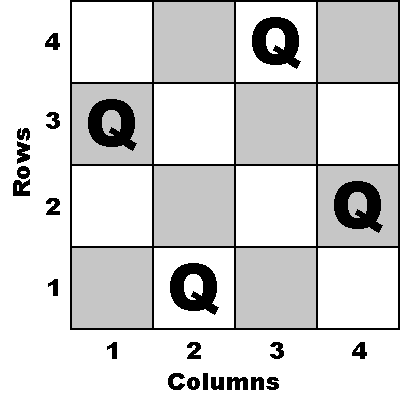
\includegraphics[width=0.7\linewidth]{../diagrams/nqueens.png}
	\caption{Example of solved 4 Queens problem.}
	\label{Nqueen fig}
\end{figure}

%\subsection{Boolean Satisfiability Problem}
%Given a boolean formula \emph{f} with considered variables \emph{V}, the Boolean Satisfiability Problem (SAT) is the problem of determining whether any state of \emph{V} satisfies \emph{f}. The SAT has been extended to many other problems due to its complex nature and due to the fact that it was the first problem proven to be NP-complete. One of the most notable problems is the 3SAT problem which contains a formula in conjuctive normal form \emph{f} containing \emph{n} clauses that are each limited to three variables \emph{x, y, z ${\in}$ V}.

%\begin{figure}[h]
%	\centering
%	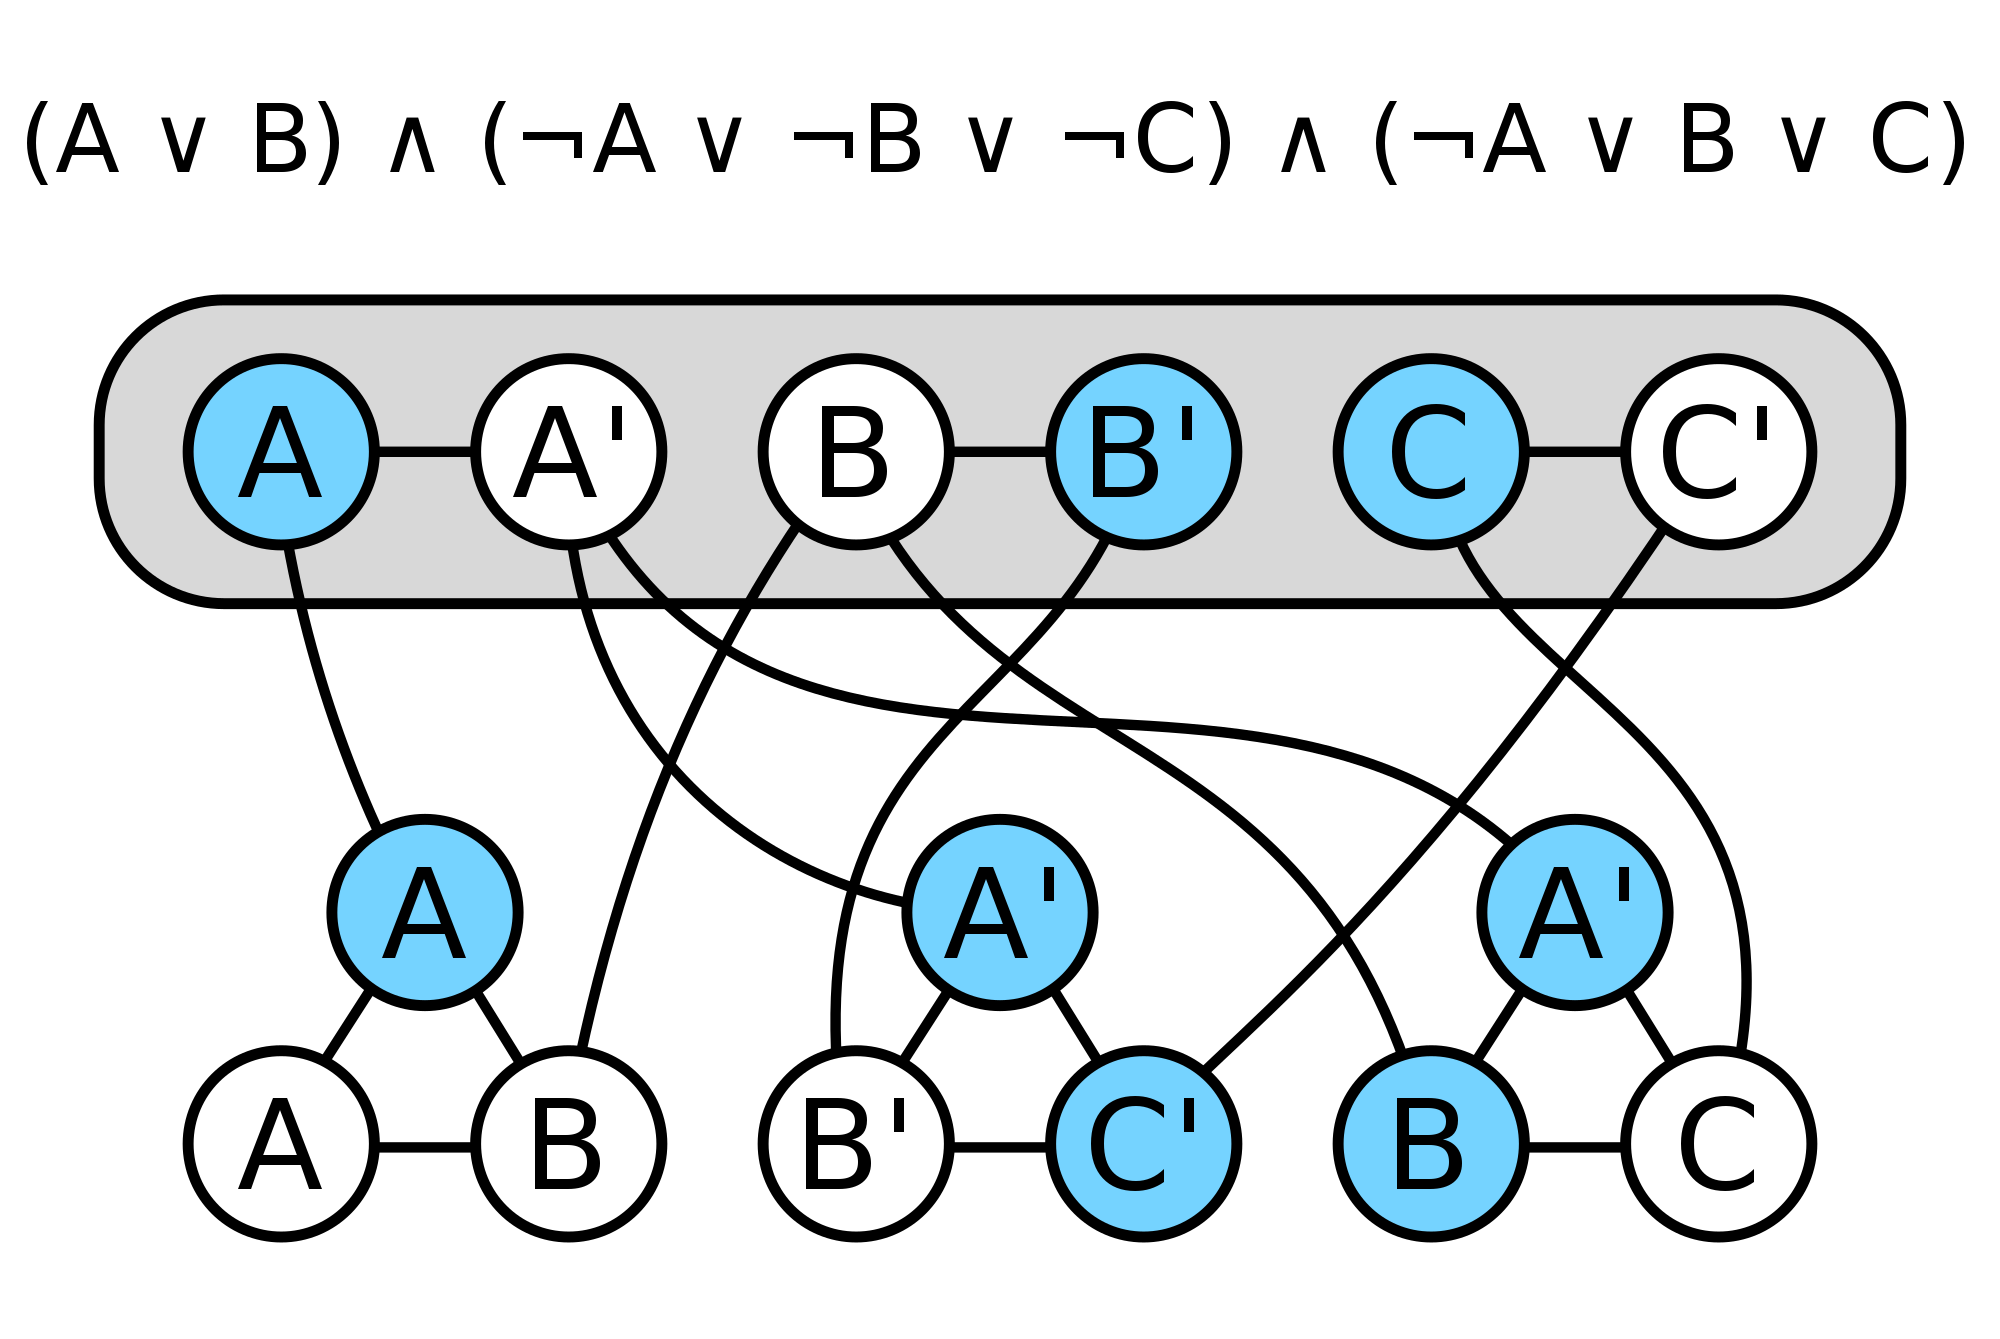
\includegraphics[width=0.7\linewidth]{../diagrams/3sat.png}
%	\caption{Example of 3SAT. As long as each clause (triangular graphs) has a path leading to an accurate value (blue colored tuple element) this problem set is satisfiable.}
%	\label{3SAT fig}
%\end{figure}

\subsection{Job Shop Scheduling Problem}
Given \emph{n} jobs and \emph{m} processors, find a distribution of job assignment that results in all jobs being completed as quickly as possible. This is the job shop scheduling problem (JSP). This problem commonly arises in optimizing computer architecture and hardware, and is a common area of study when it comes to process parallelization.This problem can be altered to any sort of schedule conflicting problem.

\begin{figure}[h]
	\centering
	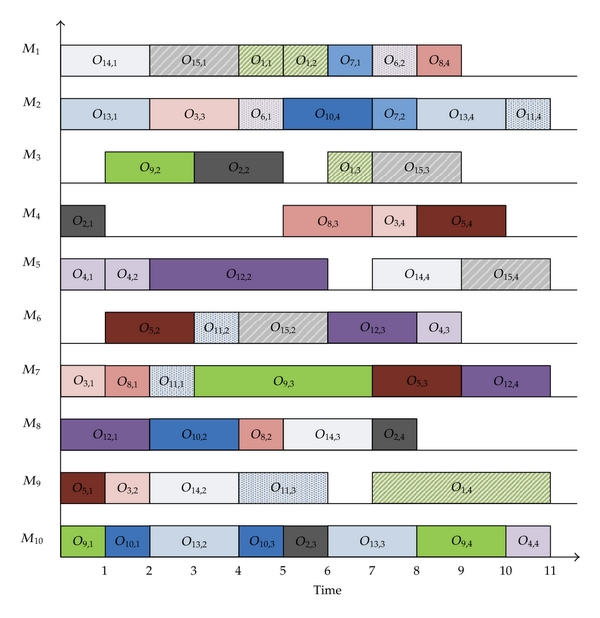
\includegraphics[width=0.7\linewidth]{../diagrams/jsp.jpg}
	\caption{$M_{x}$ is the machine. $O_{y,z}$ where $y$ is the job, and $z$ is the $z^{th}$ time this problem has been executed.}
	\label{JSS Fig}
\end{figure}

\section{Evaluation Metrics}
To evaluate our genetic algorithm we will compare heuristic variables generated with our algorithm against an algorithm with no heuristic (exhaustive) and against multiple state-of-the-art heuristics for the given problems. We will be comparing time complexity, space complexity, and accuracy to determine the effectiveness of our model. We will be testing on a single core of an Intel i5-6600k CPU @ 3.5GHz with 16gb RAM.

Time complexity will be measured in seconds, in which the lowest value is the most efficient.

Space complexity will be measured in number of vertices in the tree, in which the lowest value is the most efficient.

Accuracy will be measured by the percentage of correctness vs the most optimal solution, in which a value of 100\% is a perfect metric.

\section{Experiments} \label{Experiments}
To create a successful algorithm, we must first determine what makes a good heuristic. Due to the intense level of research done in this area, we have multiple state-of-the-art heuristics to study and learn from.

We will start by implementing a graph coloring problem and accompany it with a BnB algorithm that operates based on a heuristic function. We will then verify the sanity of our system and algorithm by running the state-of-the-art heuristics and comparing results. Similarly, we will verify that the exhaustive method of having no heuristic provides the space complexity that can be mathematically calculated.

Once the sanity of our system has been verified, we will create a genetic algorithm that will mutate the heuristic variables in an attempt to optimize results in the space, time, and accuracy areas. With our genetic algorithm in place, we will focus on increasing our algorithms performance to avoid overfitting.

We will run thousands of evolutions so that we will be able to collect enough data to accurately represent and understand the importance and value of a given problems heuristic variables.

\section{Related Work}
Considering our goal is to create an effective genetic algorithm for determining heuristic variables, a big element we need to consider is what makes certain heuristic variables more valuable than others. Meta-heuristics are heuristics that are designed to select the proper heuristic for the given problem, or to generate a new heuristic if necessary. We will be playing the role of a meta-heuristic in this paper so understanding them is vital. D.F. Jones et al. \cite{JONES20021} surveys meta-heuristics for problems that have multiple objectives. This paper states that meta-heuristics are powerful considering they can handle integer variables, discrete variables, and/or logical variables which allows for application against many problems. Non-standard goals, constraints, objectives and conditions can be easily incorporated into a meta-heuristic which even further demonstrate their flexibility.

Bektas and Tolga \cite{bektas2006multiple} survey research on the multiple traveling salesman problem (mTSP). From this survey we get an understanding of the state-of-the-art algorithms that solve mTSP, and can directly apply them to other CSPs. The authors explicitly state, ``To the best of our knowledge, no efficient heuristic algorithms exist for the solution of large-scale mTSPs" but suggest that further research on the heuristics that are known to be successful for the solution of vehicle routing problem (VRP) would be a great place to start. This gives us direction and potential for growth with our model, as we can explore solutions for similar problems to improve our model.

Bell and Stevens \cite{bell2009survey} survey the n-queens problem in great depth, even going as far as discussing theorems and multiple sub-problems. By studying both the problem and sub-problems, it helps produce an overall understanding that will help in the creation of a heuristic design to optimize these problems.

%\section{Background Work}
%TODO

\section{Research Plan}
\subsection{Challenges}
Creating an effective heuristic is challenging in itself, therefore developing a genetic algorithm that creates an effective heuristic is also going to be a big endeavor. We face a problem where if our genetic algorithm's internal heuristics aren't tuned well enough, we will run into a problem of overfitting. We will be researching different methods to ensure our genetic algorithm determines the most optimal heuristic variables.

Similarly, we face a problem where developing a fully CSP encapsulating genetic algorithm for determining heuristic variables might prove to be far too complex, considering the number and types of variables. Trying to create a clear and concise algorithm that works for every CSP is going to be incredibly difficult.

\subsection{Timeline}
The goal is to have this research ready and finished by mid April, 2019 with the possibility of extending out to the end of July, 2019. The following lays out the general plan and dates in which we want them to be completed.
\subsubsection{Phase 1}
The first phase of our research will consist of building the graph coloring problem with a BnB algorithm and applying state-of-the-art heuristics to the problem to verify the sanity of our system.

We will test the system using these state-of-the-art heuristics, as well as no heuristic to force exhaustive searches. Doing so will allow us to analyze and verify that our solution is working as intended to ensure little to no outliers when we apply our genetic algorithm.

Phase 1 will be finalized by submitting all data and analytics involved in testing the state-of-the-art and no heuristic solutions that verify the sanity of our system.

\subsubsection{Phase 2}
The second phase will focus on developing the genetic algorithm that can mutate CSP heuristic variables and test them against the graph coloring problem generated in phase 1. This phase will also consist of genetic algorithm research and how to optimize your genetic algorithm heuristic.

Data will be collected to quantify our algorithms success rate compared to existing heuristic solutions and submitted to the committee for verification.

\subsubsection{Phase 3}
Finally, we will apply our genetic algorithm to the nQueens problem as well as the job shop scheduling problem to find out if it has any major defects, and test its applicability to multiple problems. 

Data will be collected against these problems for our genetic algorithm versus the state-of-the-art, as well as no heuristic. Any issues with our algorithm that is discovered by applying it to a different CSP will be amended in this phase.

Phase 3 will be finalized by submitting all data collected for the nQueens problem and the job shop scheduling problem, as well as a comprehensive comparison chart between all three problems and the state-of-the-art to determine how transferable the algorithm is.

\subsubsection{Phase 4}
Data preparation and presentation materials will be the focus of this phase. Documenting our research in preparation for publishing. 

This phase will also be used for fixing any anomalies and determining any future application for this research.

\section{Significance of Research}
The significance of this research consists of two main facts. The first is that operations research and artificial intelligence are two booming fields in computer science. CSPs are common problems throughout these fields and by optimizing these problems at their base will result in an overall performance increase across a vast amount of research pursuits. Similarly, this research can be applied to many other areas as this genetic algorithm can likely be mutated to calculate heuristic variables for many other problems. The second significance is that heuristic based algorithms are something that influence every day life. Combine it with machine learning and you get an algorithm that will recommend Netflix movies and shows that you are going to like. Put it in a video game to make the game seem more realistic, as it learns your behaviors to throw appropriate level challenges at you. So many real-world implementations not only worry about having an effective heuristic, but evolving that heuristic over time depending on the different circumstances. This research will focus primary on creating an effective algorithm that can be used to create efficient heuristics.

\nocite{*}
\bibliographystyle{ieeetr}
\bibliography{mybib}

\end{document}
